% -*- TeX-engine: default; -*-
\documentclass[sigconf]{acmart}
\usepackage[font=footnotesize]{subcaption}
\usepackage[utf8]{inputenc}
\usepackage[T1]{fontenc}
\usepackage{url}
\usepackage{booktabs}
\usepackage{minted}
\usepackage{xcolor}
\usepackage{enumitem}
\usepackage{algorithm}
\usepackage[noend]{algpseudocode}

\usemintedstyle{friendly}

\setcopyright{rightsretained}
\acmYear{2018}
\copyrightyear{2018}
\acmConference{CoNEXT '18}{December 4--7, 2018}{Heraklion, Greece}
%\widowpenalty=100
%\clubpenalty=100
%\brokenpenalty=100

\begin{document}
\title{The eXpress Data Path: Fast Programmable Packet Processing in the Operating System Kernel}
\author{Toke Høiland-Jørgensen}
\affiliation{%
  \institution{Karlstad University}}
\email{toke@toke.dk}

\author{Jesper Dangaard Brouer}
\affiliation{%
  \institution{Red Hat}}
\email{brouer@redhat.com}

\author{Daniel Borkmann}
\affiliation{%
  \institution{Cilium.io}}
\email{daniel@cilium.io}

\author{John Fastabend}
\affiliation{%
  \institution{Cilium.io}}
\email{john@cilium.io}

\author{Tom Herbert}
\affiliation{%
  \institution{Quantonium Inc.}}
\email{tom@herbertland.com}

\author{David Ahern}
\affiliation{%
  \institution{Cumulus Networks}}
\email{dsahern@gmail.com}

\author{David Miller}
\affiliation{%
  \institution{Red Hat}}
\email{davem@redhat.com}

\renewcommand{\shortauthors}{T. Høiland-Jørgensen et al.}
\renewcommand{\shorttitle}{The eXpress Data Path}
\captionsetup{font+=small}

\hyphenation{exe-cution}

\begin{abstract}
  % Max abstract length is 200 words
  Programmable packet processing is increasingly implemented using kernel bypass
  techniques, where a userspace application takes complete control of the
  networking hardware to avoid expensive context switches between kernel and
  userspace. However, in this model the processing application has to either
  perform cumbersome re-injection of packets into the kernel, or handle all
  network traffic itself, making fast packet processing an all-or-nothing
  proposition.

  To overcome this limitation, we present the design of a novel approach to
  programmable packet processing, called the eXpress Data Path (XDP). In XDP,
  the operating system kernel itself provides a safe execution environment for
  custom packet processing applications, executed in device driver context. XDP
  has been merged into the mainline Linux kernel and provides a fully integrated
  solution working in concert with the kernel's networking stack. Applications
  are written in higher level languages such as C and compiled into custom
  byte code which the kernel statically analyses for safety, and translates into
  native instructions.

  We show that XDP achieves single-core packet processing performance as high as
  24 million packets per second, and illustrate the flexibility of the
  programming model through three example use cases: layer-3 routing, inline
  DDoS protection and layer-4 load balancing.
\end{abstract}

 \begin{CCSXML}
<ccs2012>
<concept>
<concept_id>10003033.10003034.10003038</concept_id>
<concept_desc>Networks~Programming interfaces</concept_desc>
<concept_significance>500</concept_significance>
</concept>
<concept>
<concept_id>10003033.10003099.10003102</concept_id>
<concept_desc>Networks~Programmable networks</concept_desc>
<concept_significance>500</concept_significance>
</concept>
<concept>
<concept_id>10011007.10010940.10010941.10010949</concept_id>
<concept_desc>Software and its engineering~Operating systems</concept_desc>
<concept_significance>300</concept_significance>
</concept>
</ccs2012>
\end{CCSXML}

\ccsdesc[500]{Networks~Programming interfaces}
\ccsdesc[500]{Networks~Programmable networks}
\ccsdesc[300]{Software and its engineering~Operating systems}

\keywords{XDP, BPF, Programmable Networking}
\maketitle

\section{Introduction}%
\label{sec:introduction}
High-performance packet processing in software has very tight bounds on the time
spent processing each packet. Network stacks in general purpose operating
systems are typically optimised for flexibility, which means they perform too
many operations per packet to be able to keep up with these high packet rates.
This has led to the increased popularity of special-purpose toolkits for
software packet processing, such as the Data Plane Development Kit
(DPDK)~\cite{dpdk}. Such toolkits generally bypass the operating system
completely, instead passing control of the network hardware directly to the
network application and dedicating one, or several, CPU cores exclusively to
packet processing.

The kernel bypass approach can significantly improve performance, but has the
drawback that it is more difficult to integrate with the existing system, and
applications have to re-implement a great deal of functionality otherwise
provided by the operating system network stack. In the worst case, this leads to
the need to operate two separate stacks: one to perform high-speed packet
processing and one to run normal application or container workloads. Doing so
results in increased system complexity, management and maintainability costs,
and blurs strict security boundaries otherwise enforced by the operating system
kernel. The latter is in particular problematic as infrastructure moves towards
container-based workloads coupled with orchestration systems such as Docker or
Kubernetes, where the kernel plays a dominant role in resource abstraction and
isolation.

As an alternative to the all-or-nothing kernel bypass packet processing
technique, we present a system that adds programmability directly in the
operating system networking stack in a cooperative way. This makes it possible
to perform high-speed packet processing that integrates seamlessly with existing
systems, while selectively leveraging functionality in the operating system.
This framework, called the eXpress Data Path (XDP), works by defining a limited
execution environment in the form of a virtual machine running a custom byte code
that is based on an extended version of BPF, the original BSD Packet Filter
\cite{mccanne_bsd_1993}. This environment executes custom programs directly in
the device driver context, before the kernel performs any other packet processing
tasks. The kernel also ensures the safety of the program by statically verifying
it before it is loaded; and programs are dynamically compiled into native machine
instructions to ensure high performance.

XDP has been gradually integrated into the Linux kernel over several releases,
but no complete architectural description of the system as a whole has been
presented before. In this work we present a high-level design description of XDP
and its capabilities, and how it integrates with the rest of the Linux kernel.
Our performance evaluation shows raw packet processing performance of up to 24
million packets per second per CPU core. While this does not quite match the
highest achievable performance in a DPDK-based application on the same hardware,
we argue that the XDP system makes up for this by offering several compelling
advantages over DPDK and other kernel bypass solutions. Specifically, XDP:

\begin{itemize}
\item Integrates cooperatively with the regular networking stack, retaining full
  control of the hardware in the kernel. This retains the kernel security
  boundary, and requires no changes to network configuration and management
  tools. In addition, any network adapter with a Linux driver can be supported
  by XDP; no special hardware features are needed, and drivers need not be
  re-implemented from scratch.

\item Makes it possible to selectively utilise kernel network stack features
  such as the routing table and TCP stack, keeping the same configuration
  interface while accelerating critical performance paths.

\item Provides a stable programming interface (API) for packet processing
  applications, which carries the same stability guarantees as the kernel system
  call interface.

\item Does not require expensive packet re-injection from user space into kernel
  space when interacting with workloads based on the normal socket layer.

\item Is transparent to applications running on the host, enabling new
  deployment scenarios such as inline protection against denial of service
  attacks on servers.

\item Can be dynamically re-programmed without any service interruption, which
  means that features can be added on the fly or removed completely when they
  are not needed without interruption of network traffic, and that processing
  can react dynamically to conditions in other parts of the system.

\item Does not require dedicating full CPU cores to packet processing, which
  means lower traffic levels translate directly into lower CPU usage. This has
  important efficiency and power saving implications.
\end{itemize}

In the rest of this paper we present the design of XDP and our performance
analysis. This is structured as follows: Section~\ref{sec:related-work} first
outlines related work. Section~\ref{sec:design} then presents the design of the
XDP system and Section~\ref{sec:perf-eval} presents our evaluation of its raw
packet processing performance. Section~\ref{sec:usecases} supplements this with
examples of real-world use cases that can be implemented with XDP. Finally,
Section~\ref{sec:limitations} presents some known limitations of XDP and future
work to address them, and Section~\ref{sec:conclusion} concludes.

\section{Related Work}%
\label{sec:related-work}

XDP is certainly not the first system enabling programmable packet processing.
Rather, this field has gained momentum over the last several years, and
continues to do so. Several frameworks have been presented to enable this kind
of programmability, and they have enabled many novel applications. Examples of
such applications include those performing single functions, such as
switching~\cite{rizzo2012vale}, routing~\cite{han2010packetshader}, named-based
forwarding~\cite{kirchner2016augustus}, classification~\cite{santiago2012wire},
caching~\cite{mansilha2015hierarchical} or traffic
generation~\cite{emmerich2015moongen}. They also include more general solutions
which are highly customisable and can operate on packets from a variety of
sources~\cite{han2012megapipe,marian2012netslices,linguaglossa2017high,morris1999click,dobrescu2009routebricks,openvswitch}.

To achieve high packet processing performance on Common Off The Shelf (COTS)
hardware, it is necessary to remove any bottlenecks between the networking
interface card (NIC) and the program performing the packet processing. Since one
of the main sources of performance bottlenecks is the interface between the
operating system kernel and the userspace applications running on top of it
(because of the high overhead of a system call and complexity of the underlying
feature-rich and generic stack), low-level packet processing frameworks have to
manage this overhead in one way or another. The existing frameworks, which have
enabled the applications mentioned above, take several approaches to ensuring
high performance; and XDP builds on techniques from several of them. In the
following we give a brief overview of the similarities and differences between
XDP and the most commonly used existing frameworks.

The DataPlane Development Kit (DPDK)~\cite{dpdk} is probably the most widely
used framework for high-speed packet processing. It started out as an
Intel-specific hardware support package, but has since seen a wide uptake under
the stewardship of the Linux Foundation. DPDK is a so-called \emph{kernel
  bypass} framework, which moves the control of the networking hardware out of
the kernel into the networking application, completely removing the overhead of
the kernel-userspace boundary. Other examples of this approach include the
PF\_RING ZC module~\cite{pfringzc} and the hardware-specific Solarflare
OpenOnload~\cite{openonload}. Kernel bypass offers the highest performance of
the existing frameworks~\cite{gallenmuller_comparison_2015}; however, as
mentioned in the introduction, it has significant management, maintenance and
security drawbacks.

XDP takes an approach that is the opposite of kernel bypass: Instead of moving
control of the networking hardware \emph{out} of the kernel, the
performance-sensitive packet processing operations are moved \emph{into} the
kernel, and executed before the operating system networking stack begins its
processing. This retains the advantage of removing the kernel-userspace boundary
between networking hardware and packet processing code, while keeping the kernel
in control of the hardware, thus preserving the management and security
guarantees offered by the operating system. The key innovation that enables this
is the use of a virtual execution environment that verifies that loaded programs
will not harm or crash the kernel.

% Should Juniper Contrail vRouter be mentioned below? It is not a 'prominent' or
% well known example, but their Linux approach is loading a kernel module.
%
Prior to the introduction of XDP, implementing packet processing functionality
as a kernel module has been a high-cost approach, since mistakes can crash the
whole system, and internal kernel APIs are subject to frequent change. For this
reason, it is not surprising that few systems have taken this approach. Of those
that have, the most prominent examples are the OpenVswitch~\cite{openvswitch}
virtual switch and the Click~\cite{morris1999click} virtual router framework,
which are both highly configurable systems with a wide scope, allowing them to
amortise the cost over a wide variety of uses. XDP significantly lowers the cost
for applications of moving processing into the kernel, by providing a safe
execution environment, and by being supported by the kernel community, thus
offering the same API stability guarantee as every other interface the kernel
exposes to userspace. In addition, XDP programs can completely bypass the
networking stack, which offers higher performance than a traditional kernel
module that needs to hook into the existing stack.

While XDP allows packet processing to move into the operating system for maximum
performance, it also allows the programs loaded into the kernel to selectively
redirect packets to a special user-space socket type, which bypasses the normal
networking stack, and can even operate in a zero-copy mode to further lower the
overhead. This operating mode is quite similar to the approach used by
frameworks such as Netmap~\cite{rizzo2012netmap} and
PF\_RING~\cite{deri2009modern}, which offer high packet processing performance
by lowering the overhead of transporting packet data from the network device to
a userspace application, without bypassing the kernel completely. The Packet I/O
engine that is part of PacketShader~\cite{han2010packetshader} is another
example of this approach, and it has some similarities with special-purpose
operating systems such as Arrakis~\cite{peter2016arrakis} and
ClickOS~\cite{martins2014clickos}.

Finally, programmable hardware devices are another way to achieve
high-performance packet processing. One example is the
NetFPGA~\cite{lockwood2007netfpga}, which exposes an API that makes it possible
to run arbitrary packet processing tasks on the FPGA-based dedicated hardware.
The P4 language~\cite{bosshart2014p4} seeks to extend this programmability to a
wider variety of packet processing hardware (including, incidently, an XDP
backend~\cite{p4xdp}). In a sense, XDP can be thought of as a ``software
offload'', where performance-sensitive processing is offloaded to increase
performance, while applications otherwise interact with the regular networking
stack. In addition, XDP programs that don't need to access kernel helper
functions can be offloaded entirely to supported networking hardware (currently
supported with Netronome smart-NICs~\cite{xdp-offload}).

In summary, XDP represents an approach to high-performance packet processing
that, while it builds on previous approaches, offers a new tradeoff between
performance, integration into the system and general flexibility. The next
section explains in more detail how XDP achieves this.

\section{The design of XDP}
\label{sec:design}

\begin{figure}[t]
\centering
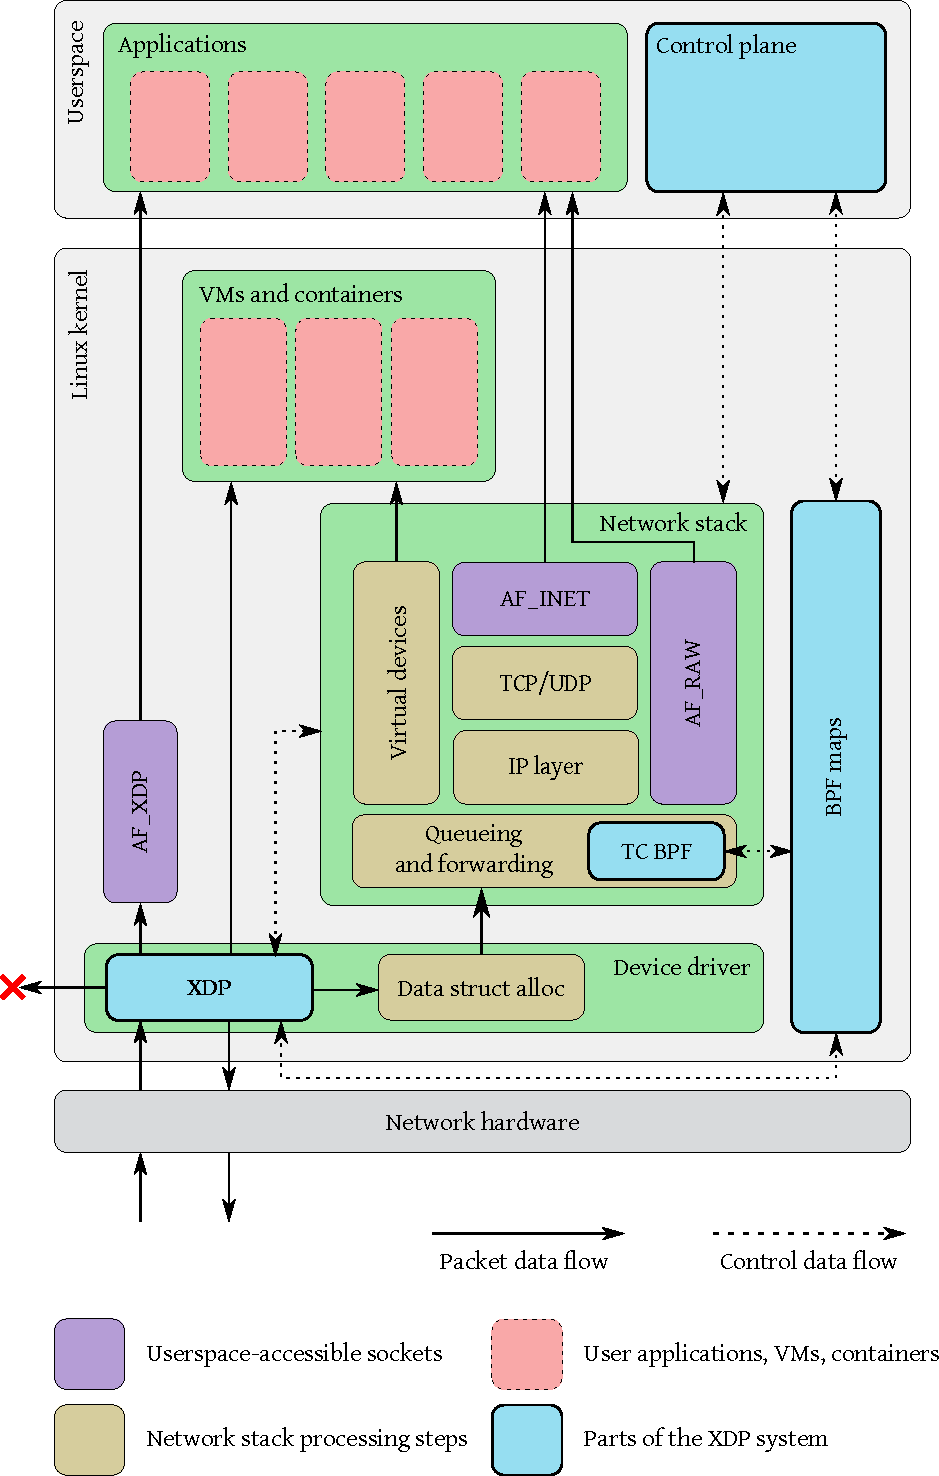
\includegraphics[width=\linewidth]{figures/kernel-diagram.pdf}
\caption{\label{fig:xdp-kernel} XDP's integration with the Linux network stack.}
\end{figure}

\begin{figure*}[t]
\centering
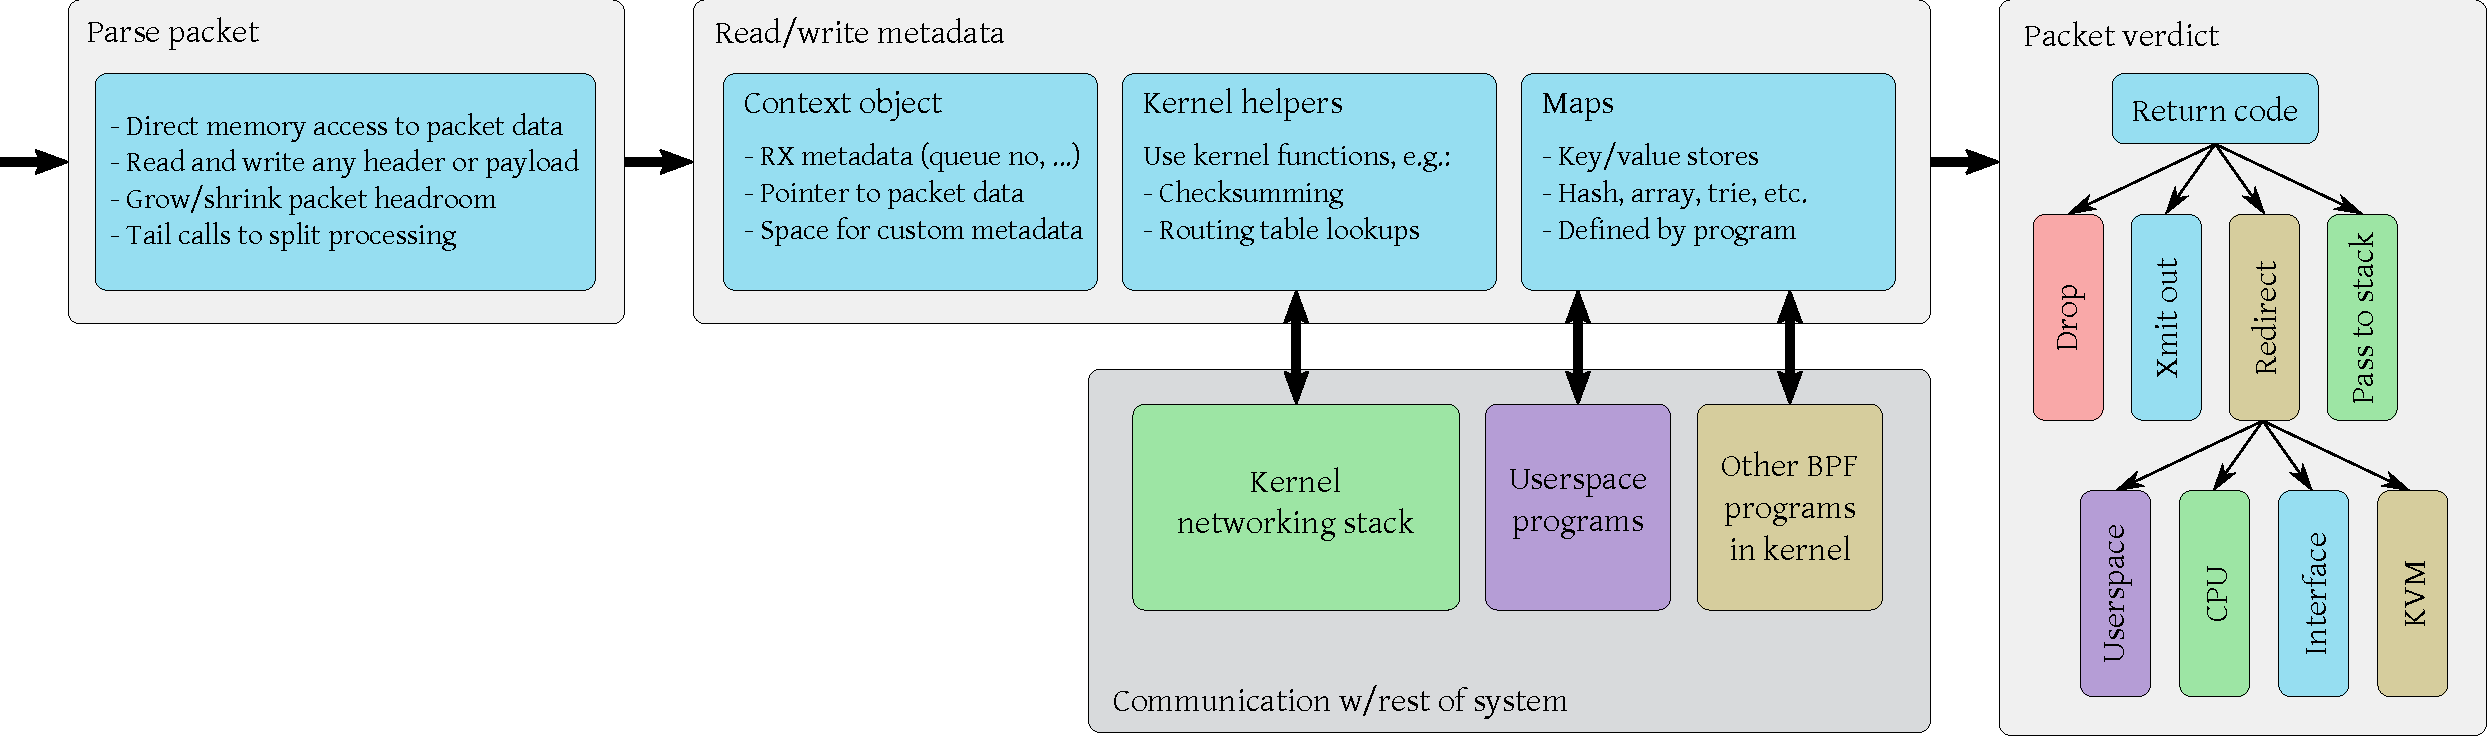
\includegraphics[width=\linewidth]{figures/xdp-execution-diagram.pdf}
\caption{\label{fig:xdp-execution} Execution flow of a typical XDP program. When
  a packet arrives, the program starts by parsing packet headers to extract the
  information it will react on. It then reads or updates metadata from one of
  several sources. Finally, a packet can be rewritten and a final verdict for
  the packet is determined. The program can alternate between packet parsing,
  metadata lookup and rewriting, all of which are optional. The final verdict is
  given in the form of a program return code.}
\end{figure*}



The driving rationale behind the design of XDP has been to allow
high-performance packet processing that can integrate cooperatively with the
rest of the kernel, while ensuring the safety and integrity of the rest of the
system. Thus, XDP integrates deeply with the Linux kernel, making it possible to
perform custom packet processing while taking advantage of the extensive feature
set of the operating system. This deep integration with the kernel obviously
imposes some design constraints, and the components of XDP have been gradually
introduced into the Linux kernel over a number of releases, and the design has
been informed by the feedback and testing obtained during this process.

Unfortunately, recounting the process and lessons learned is not possible in the
scope of this paper. Instead, this section describes the complete system, by
explaining how the major components of XDP work, and how they fit together to
create the full system. This is illustrated by Figure~\ref{fig:xdp-kernel},
which shows a diagram of how XDP integrates into the Linux kernel, and
Figure~\ref{fig:xdp-execution}, which shows the execution flow of a typical XDP
program. There are four major components of the XDP system:

\begin{itemize}
\item \textbf{The XDP driver hook} is the main entry point for an XDP program,
  and is executed when a packet is received from the hardware.

\item \textbf{The eBPF virtual machine} executes the byte code of the XDP
  program, and just-in-time-compiles it for increased performance.

\item \textbf{BPF maps} are key/value stores that serve as the primary
  communication channel to the rest of the system.

\item \textbf{The eBPF verifier} statically verifies programs before they are
  loaded to make sure they do not crash or corrupt the running kernel.
\end{itemize}


\subsection{The XDP Driver Hook}
\label{sec:prog-model}


An XDP program is run by a hook in the network device driver each time a packet
arrives. The infrastructure to execute the program is contained in the kernel as
a library function, which means that the program is executed directly in the
device driver, without context switching to userspace. As shown in
Figure~\ref{fig:xdp-kernel}, the program is executed at the earliest possible
moment after a packet is received from the hardware, before the kernel allocates
its per-packet \emph{sk\_buff} data structure or performs any parsing of the
packet.

Figure~\ref{fig:xdp-execution} shows the various processing steps typically
performed by an XDP program. The program starts its execution with access to a
context object. This object contains pointers to the raw packet data, along with
metadata fields describing which interface and receive queue the packet was
received on, etc.

The program typically begins by parsing packet data, and can pass control to a
different XDP program through tail calls, thus splitting processing into
logical sub-units (based on, say, IP header version).

After parsing the packet data, the XDP program can read or write metadata
associated with the packet. This is accessible through the context object, which
contains read-only metadata fields as well as a pointer to a special memory area
that XDP programs can use to store its own arbitrary metadata. The latter will
be available to other XDP programs, as well as to other parts of the kernel and
userspace.
% This metadata area is placed inline in packet payload, just before packet
% headers.
%
Additionally, an XDP program has access to kernel facilities that
provide additional metadata through helper functions and maps (dotted lines in
Figure~\ref{fig:xdp-kernel} and the top part of Figure~\ref{fig:xdp-execution}).
New helper functions are actively added by the kernel development community in
response to user requests, continuously expanding the functionality that XDP
programs can make use of.

Finally, the program can write any parts of the packet data buffer, including
expanding or shrinking the packet to add or remove headers. This allows it to
perform encapsulation or decapsulation, as well as, for instance, rewrite
address fields for forwarding. Various kernel helper functions are available to
assist with things like checksum calculation for a modified packet.

These three steps (reading, metadata processing, and writing packet data)
correspond to the light grey boxes on the left side of
Figure~\ref{fig:xdp-execution}. Since XDP programs can contain arbitrary
instructions, the different steps can alternate and repeat in arbitrary ways.
However, to achieve high performance, it is often necessary to structure the
execution order as described here.

At the end of processing, the XDP program issues a final verdict for the packet.
This is done by way of a program return code, which is shown on the right-hand
side of Figure~\ref{fig:xdp-execution}. There are three simple return codes
which either drops the packet, immediately re-transmits it out the same network
interface, or allows the packet to be processed by the kernel networking stack.
In addition to these simple actions, the XDP program can \emph{redirect} the
packet, which offers additional control over its further processing.

The redirect facility is designed as a flexible forwarding mechanism. It uses
BPF maps to store the redirect targets, which allows the targets to be
dynamically updated from userspace. Currently, redirecting can be used (1) to
transmit the raw packet out a different network interface (including virtual
interfaces connected to virtual machines), (2) to pass it to a different CPU for
further processing, or (3) to pass it directly to a special userspace socket
address family (\texttt{AF\_XDP}). These different packet paths are shown as
solid lines in Figure~\ref{fig:xdp-kernel}. The flexibility of the forwarding
mechanism means that it can be extended with additional target types without
requiring any special support from either the XDP programs themselves, or the
device drivers implementing the XDP hooks.

\subsection{The eBPF Virtual Machine}
\label{sec:bpf-vm}
XDP programs run in the Extended BPF (eBPF) virtual machine. eBPF is an
evolution of the original BSD packet filter (BPF) \cite{mccanne_bsd_1993} which
has seen extensive use in various packet filtering applications over the last
decades. BPF uses a register-based virtual machine to describe filtering
actions. The BPF virtual machine has two 32-bit registers and understands 22
different instructions. This makes it well suited for packet filtering
operations, but limited as a general purpose virtual machine. eBPF extends the
original BPF virtual machine to allow full general purpose execution and
efficient just-in-time (JIT) compilation into native machine code. Support for
compiling (restricted) C code into eBPF is included in the LLVM compiler
infrastructure~\cite{llvm}.

The verifier (described in Section~\ref{sec:bpf-verifier} below) ensures that
user-supplied programs cannot harm the running kernel. With this in place, it is
safe to execute the code directly in the kernel address space, which makes eBPF
useful for a wide variety of tasks in the Linux kernel, of which XDP is one.
Apart from the XDP driver hook, eBPF is used for packet processing in the
Traffic Control (TC) subsystem, where programs can filter packets after they
have been parsed by the kernel, or before they are passed to the hardware from
applications. This is marked as ``TC BPF'' in Figure~\ref{fig:xdp-kernel}. In
addition, eBPF programs can be attached to various places in the kernel that are
unrelated to networking (not shown in the figures). Because all eBPF programs
can share the same set of maps, this makes it possible for programs to react to
arbitrary events in other parts of the kernel. For instance, an XDP program
could drop packets if CPU load increases above a certain threshold.

At the instruction set level, eBPF extends the original BPF virtual machine by
adding more registers and more instructions. The number of registers is
increased from two to eleven, and register widths are increased to 64 bits. The
64-bit registers map one-to-one to hardware registers on the 64-bit
architectures supported by the kernel, which eases JIT compilation.

The added instructions are primarily arithmetic and logic instructions that
allows efficient manipulation of the larger register sizes. In addition to this,
eBPF adds a \emph{call} instruction for function calls, and adopts the same
calling convention as the C language conventions used on the architectures
supported by the kernel. Along with the register mapping mentioned above, this
makes it possible to map a BPF call instruction to a single native call
instruction, enabling function calls with close to zero additional overhead.
This facility is used by eBPF to support helper functions that eBPF programs can call to
interact with the kernel while processing, as well as for function calls within
the same eBPF program.

The eBPF virtual machine supports dynamically loading and re-loading programs,
and the kernel manages the life cycle of all programs. This makes it possible to
extend or limit the amount of processing performed for a given situation, by
adding or completely removing parts of the program that are not needed, and
re-loading it atomically as requirements change. The dynamic loading of programs
also makes it possible to express processing rules directly in program code,
avoiding any data structure lookups needed by more generic code.

\subsection{BPF Maps}
\label{sec:bpf-maps}
eBPF programs are executed in response to an event in the kernel (a packet
arrival, in the case of XDP). Each time they are executed they start in the same
initial state, and they do not have access to persistent memory storage in their
program context. Instead, programs can access \emph{BPF maps}.

BPF maps are key/value stores that are defined upon loading an eBPF program, and
can be referred to from within the eBPF code. Maps exist in both global and
per-CPU variants, and can be shared, both between different eBPF programs
running at various places in the kernel, as well as between eBPF and userspace.
The map types include generic hash maps, arrays and radix trees, as well as
specialised types containing pointers to eBPF programs (used for tail calls), or
redirect targets, or even recursive pointers to other maps.

Maps serve several purposes: they are a persistent data store between
invocations of the same eBPF program; a global coordination tool, where eBPF
programs in one part of the kernel can update state that changes the behaviour
in another; and a communication mechanism between userspace programs and the
kernel eBPF programs, similar to the communication between control plane and
data plane in other programmable package processing systems.

\subsection{The eBPF Verifier}
\label{sec:bpf-verifier}
Since eBPF code runs directly in the kernel address space, it can directly
access, and potentially corrupt, arbitrary kernel memory. To prevent this from
happening, the kernel enforces a single entry point for loading all eBPF
programs (through the \texttt{bpf()} system call). When loading an eBPF program
it is first analysed by the in-kernel eBPF verifier. The verifier performs a
static analysis of the program byte code to ensure that the program performs no
actions that are unsafe (such as accessing arbitrary memory), and that the
program will terminate. The latter is ensured by disallowing loops and limiting
the maximum program size. The verifier works by first building a directed
acyclic graph (DAG) of the control flow of the program. This DAG is then
verified as follows:

First, the verifier performs a depth-first search on the DAG to ensure it is in
fact acyclic, i.e., that it contains no loops, and also that it contains no
unsupported or unreachable instructions. Then, in a second pass, the verifier
walks all possible paths of the DAG. The purpose of this second pass is to
ensure that the program performs only safe memory accesses, and that any helper
functions are called with the right argument types. This is ensured by rejecting
programs that perform load or call instructions with invalid arguments. Argument
validity is determined by tracking the state of all registers and stack
variables through the execution of the program.

\begin{listing}[p]
  \caption{\label{lst:ex-xdp-prog}Example XDP program. The program parses packet
    headers, swaps source and destination MAC addresses for all UDP packets, and
    sends them back out the same interface. A packet counter is kept per IP
    protocol number. Adapted from xdp2\_kern.c, which is distributed with the
    kernel source code.}
\begin{minted}[linenos,fontsize=\footnotesize,tabsize=3]{c}
/* map used to count packets; key is IP protocol, value is pkt count */
struct bpf_map_def SEC("maps") rxcnt = {
	.type = BPF_MAP_TYPE_PERCPU_ARRAY,
	.key_size = sizeof(u32),
	.value_size = sizeof(long),
	.max_entries = 256,
};

/* swaps MAC addresses using direct packet data access */
static void swap_src_dst_mac(void *data)
{
	unsigned short *p = data;
	unsigned short dst[3];
	dst[0] = p[0];   dst[1] = p[1];   dst[2] = p[2];
	p[0]   = p[3];   p[1]   = p[4];   p[2]   = p[5];
	p[3]   = dst[0]; p[4]   = dst[1]; p[5]   = dst[2];
}

static int parse_ipv4(void *data, u64 nh_off, void *data_end)
{
	struct iphdr *iph = data + nh_off;
	if (iph + 1 > data_end)
		return 0;
	return iph->protocol;
}

SEC("xdp1") /* marks main eBPF program entry point */
int xdp_prog1(struct xdp_md *ctx)
{
	void *data_end = (void *)(long)ctx->data_end;
	void *data = (void *)(long)ctx->data;
	struct ethhdr *eth = data; int rc = XDP_DROP;
	long *value; u16 h_proto; u64 nh_off; u32 ipproto;

	nh_off = sizeof(*eth);
	if (data + nh_off > data_end)
		return rc;

	h_proto = eth->h_proto;

	/* check VLAN tag; could be repeated to support double-tagged VLAN */
	if (h_proto == htons(ETH_P_8021Q) || h_proto == htons(ETH_P_8021AD)) {
		struct vlan_hdr *vhdr;

		vhdr = data + nh_off;
		nh_off += sizeof(struct vlan_hdr);
		if (data + nh_off > data_end)
			return rc;
		h_proto = vhdr->h_vlan_encapsulated_proto;
	}

	if (h_proto == htons(ETH_P_IP))
		ipproto = parse_ipv4(data, nh_off, data_end);
	else if (h_proto == htons(ETH_P_IPV6))
		ipproto = parse_ipv6(data, nh_off, data_end);
	else
		ipproto = 0;

	/* lookup map element for ip protocol, used for packet counter */
	value = bpf_map_lookup_elem(&rxcnt, &ipproto);
	if (value)
		*value += 1;

	/* swap MAC addrs for UDP packets, transmit out this interface */
	if (ipproto == IPPROTO_UDP) {
		swap_src_dst_mac(data);
		rc = XDP_TX;
	}
	return rc;
}

\end{minted}
\end{listing}

The purpose of this register state tracking mechanism is to ensure that the
program performs no out of bounds memory accesses \emph{without knowing in
  advance what the valid bounds are}. The bounds cannot be known because
programs must process data packets which vary in size; and similarly, the
contents of maps are not known in advance, so it is not known whether a given
lookup will succeed.

One way to deal with this problem is to automatically generate bounds checking
code around all memory accesses. However, the eBPF verifier takes a different
approach, which leaves more control in the hands of the eBPF program writers: It
verifies that the program being loaded does its own bounds checking before
dereferencing pointers to packet data, and that map lookups are checked for
\texttt{NULL} values before being dereferenced. With this verification in place,
it is safe for program instructions to directly access packet data, which is an
important reason for the high performance of eBPF packet processing programs.

To track data access, the verifier tracks data types, pointer offsets and value
ranges of all registers. At the beginning of the program, \texttt{R1} contains a
pointer to the execution context, \texttt{R10} is a stack pointer, and all other
registers are marked as not initialised. At each execution step, register states
are updated based on the operations performed by the program. When a new value
is stored in a register, that register inherits the state variables from the
source of the value. Arithmetic operations will affect the possible value ranges
of scalar types, and the offset of pointer types. The widest possible range is
stored in the state variables, e.g., if a one-byte load is performed into a
register, that register's possible value range is set to 0-255. Branches in the
instruction graph will update the register state according to the logical
operation contained in the branch. For example, given a comparison such as
"\texttt{R1 > 10}", the verifier will set the maximum value of \texttt{R1} to 10
in one branch, and the minimum value to 11 in the other.

Using this range information stored in the state variables, it is possible for
the verifier to predict the ranges of memory that each load instruction can
potentially access, and ensure that only safe memory accesses are performed. For
packet data access this is done by looking for comparisons with the special
\texttt{PACKET\_END} pointer that is available in the execution context; for
values retrieved from a BPF map the data size in the map definition is used; and
for values stored on the stack, accesses are checked against the data ranges
that have previously been written to. Any eBPF program that makes memory
accesses that the verifier cannot prove are safe, are simply rejected at load
time. In addition to this, the verifier also uses the range information to
enforce aligned memory accesses.

It should be noted that the purpose of the verifier is to protect the internals
of the kernel from being exposed to malicious or buggy eBPF programs, not to
ensure that the programs perform their designated function in the most efficient
way possible. That is, an XDP program can slow down the machine by performing
excessive processing (up to the maximum program size), and it can corrupt
network packets if written incorrectly. Loading programs requires administrative
(root) privileges for this reason, and it is up to the eBPF programmer to
prevent these types of bugs, and to the system administrator to decide which
programs to load on the system.


\subsection{Example XDP program}
\label{sec:example-xdp-program}


To showcase the features described above, Listing~\ref{lst:ex-xdp-prog} shows an
example of a simple XDP program. The program will parse packet headers, and
reflect all UDP packets by swapping the source and destination MAC addresses and
sending the packet back out the interface it came in on. While this is obviously
a very simple example, the program does feature most of the components of an XDP
program that is useful in the real world. Specifically:

\begin{itemize}
\item A BPF map is defined (lines 1--7) for keeping statistics of the number of
  processed packets. The map is keyed on IP protocol number and each value is
  simply a packet count (updated in lines 60--62). A userspace program can poll
  this map to output statistics while the XDP program is running.
\item Pointers to the start and end of the packet data is read from the context
  object (lines 30--31), to be used for direct packet data access.
\item Checking against the data\_end pointer ensures that no data is read out of
  bounds (lines 22, 36 and 47). The verifier ensures correctness even across
  pointer copies (as in lines 21--22).
\item The program must handle any packet parsing itself, including things such
  as VLAN headers (lines 41--50).
\item Direct packet data access is used to modify the packet headers (lines
  14--16).
\item The map lookup helper functions exposed by the kernel (called on line 60).
\item The final packet verdict is communicated by the program return code (line
  69).
\end{itemize}


When the program is installed on an interface, it is first compiled into eBPF
byte code, then checked by the verifier. The notable things checked by the
verifier in this case are (a) the absence of loops, and the total size of the
program, (b) that all direct packet data accesses are preceded by appropriate
bounds checking (c) that the sizes of parameters passed to the map lookup
function matches the map definition, and (d) that the return value from the map
lookup is checked against NULL before it is accessed.


\subsection{Summary}
\label{sec:design-summary}

The XDP system consists of four major components: (1) The XDP device driver hook
which is run directly after a packet is received from the hardware. (2) The eBPF
virtual machine which is responsible for the actual program execution (and is
also used for executing programs in other parts of the kernel). (3) BPF maps,
which allow programs running in various parts of the kernel to communicate with
each other and with userspace. And (4) The eBPF verifier, which ensures programs
do not perform any operations that can harm the running kernel.

These four components combine to create a powerful environment for writing
custom packet processing applications, that can accelerate packet processing in
essential paths, while integrating with the kernel and making full use of its
existing facilities. The performance achievable by these applications is the
subject of the next section.

\section{Performance evaluation}
\label{sec:perf-eval}
In this section we present our performance evaluation of XDP. As mentioned in
Section~\ref{sec:related-work}, there are quite a few existing systems for
high-performance packet processing, and benchmarking all of them is not feasible
in the scope of this paper. Instead, we note that DPDK is the existing solution
that achieves the highest performance~\cite{gallenmuller_comparison_2015}, and
compare against that as a baseline for the current state of the art in
high-speed software packet processing (using the \texttt{testpmd} example
application shipped with the 18.05 release of DPDK). We focus on the raw packet
processing performance, using synthetic benchmarks, and also compare against the
performance of the Linux kernel network stack, to show the performance
improvements offered by XDP in the same system. In the next section, we
supplement these raw performance benchmarks with some examples of real-world
applications implemented on top of XDP, to demonstrate their feasibility within
the programming model.

For all benchmarks, we use a machine equipped with a hexa-core Intel Xeon
E5-1650 v4 CPU running at 3.60GHz, which supports Intel's Data Direct I/O (DDIO)
technology allowing the networking hardware Direct Memory Access (DMA) system to
place packet data directly in the CPU cache. The test machine is equipped with
two Mellanox ConnectX-5 Ex VPI dual-port 100Gbps network adapters, which are
supported by the \emph{mlx5} driver. We use the TRex packet
generator~\cite{cisco18:_trex_traff_gener} to produce the test traffic. The test
machine runs a pre-release of version 4.18 of the Linux kernel. To help others
reproduce our results, we make available the full details of our setup, along
with links to source code and the raw test data, in an online
repository~\cite{test-data}.

In our evaluation, we focus on three metrics:

\begin{itemize}
\item Packet drop performance. To show the maximum packet processing
  performance, we measure the performance of the simplest possible operation of
  dropping the incoming packet. This effectively measures the overhead of the
  system as a whole, and serves as an upper bound on the expected performance of
  a real packet processing application.

\item CPU usage. As mentioned in the introduction, one of the benefits of XDP is
  that it scales the CPU usage with the packet load, instead of dedicating CPU
  cores exclusively to packet processing. We quantify this by measuring how CPU
  usage scales with the offered network load.

\item Packet forwarding performance. A packet processing system that cannot
  forward packets has limited utility. Since forwarding introduces an additional
  complexity compared to the simple processing case (e.g., interacting with more
  than one network adapter, rewriting link-layer headers, etc.), a separate
  evaluation of forwarding performance is useful. We include both throughput and
  latency in the forwarding evaluation.
\end{itemize}

We have verified that with full-sized (1500 bytes) packets, our system can
process packets at line-speed (100\,Gbps) on a single core that is half-idle.
This makes it clear that the challenge is processing many \emph{packets} per
second, as others have also noted~\cite{rizzo2012netmap}. For this reason, we
perform all tests using minimum-sized (64 bytes) packets, and measure the
maximum number of packets per second the system can process. To measure how
performance scales with the number of CPU cores, we repeat the tests with an
increasing number of cores dedicated to packet processing.\footnote{The
  Hyperthreading feature of the CPU is disabled for our experiments, so whenever
  we refer to the number of active CPU cores, this means the number of physical
  cores.} For XDP and the Linux network stack (which do not offer an explicit
way to dedicate cores to packet processing) we achieve this by configuring the
hardware Receive Side Scaling (RSS) feature to steer traffic to the desired
number of cores for each test.

As we will see in the results below, our tests push the hardware to its very
limits. As such, tuning the performance of the system as a whole is important to
realise optimal performance. This includes the physical hardware configuration,
configuration of the network adapter features such as Ethernet flow control and
receive queue size, and configuration parameters of the Linux kernel, where we
for instance disable full preemption and the ``retpoline'' mitigation for the
recent Meltdown and Spectre vulnerabilities. The full details of these
configuration issues are omitted here due to space constraints, but are
available in the online repository.

The following subsections present the evaluation results for each of the metrics
outlined above, followed by a general discussion of the performance of XDP
compared to the other systems. As all our results are highly repeatable, we show
results from a single test run (with no error bars) to make the graphs more
readable.

\subsection{Packet Drop Performance}
\label{sec:basel-pack-proc}

\begin{figure}[t]
\centering
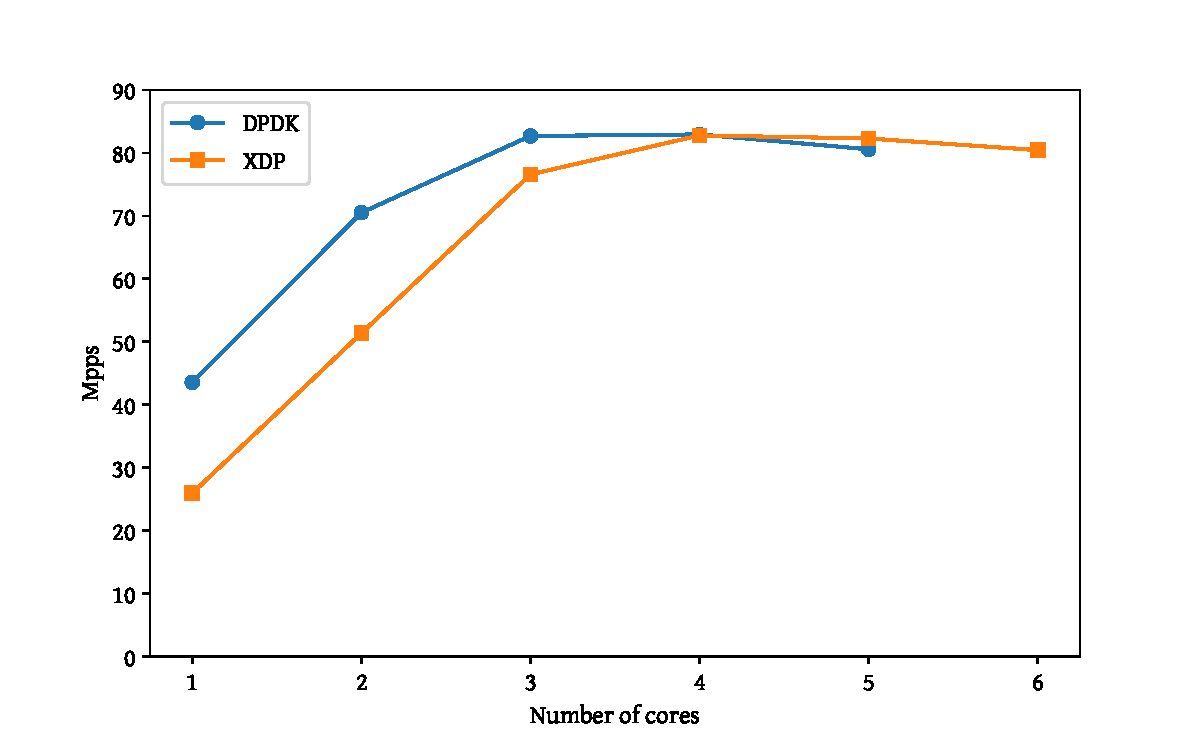
\includegraphics[width=\linewidth]{figures/drop-test.pdf}
\caption{\label{fig:drop-test} Packet drop performance. DPDK uses one core for
  control tasks, so only 5 are available for packet processing.}
\end{figure}

Figure~\ref{fig:drop-test} shows the packet drop performance as a function of
the number of cores. The baseline performance of XDP for a single core is
24\,Mpps, while for DPDK it is 43.5\,Mpps. Both scale their performance linearly
up to the global performance limit of the PCI bus, which is reached at 115\,Mpps
after enabling PCI descriptor compression support in the hardware (which trades
CPU cycles for PCI bus bandwidth).


The figure also shows the performance of the Linux networking stack in two
configurations: one where we use the ``raw'' table of the \emph{iptables}
firewall module to drop packets, which ensures the earliest possible drop in the
network stack processing; and another where we use the connection tracking
(\emph{conntrack}) module, which is enabled by default on many Linux
distributions, but which carries a high overhead. These two modes illustrate the
performance span of the Linux networking stack, from 1.8 Mpps of single-core
performance with conntrack, up to 4.8 Mpps in raw mode. It also shows that in
the absence of hardware bottlenecks, Linux performance scales linearly with the
number of cores. And finally, it shows that with its 24 Mpps on a single core,
XDP offers a five-fold improvement over the fastest processing mode of the
regular networking stack.

As part of this test, we also measured the overhead of the Linux raw mode
dropping performance from installing an XDP program that does no operation other
than pass the packet on to the stack. We measured a drop in performance to
4.5\,Mpps on a single core, corresponding to 13.3\,ns of processing overhead.
This is not shown on the figure, because the difference is too small to be
legible.

\subsection{CPU Usage}
\label{sec:cpu-usage}

The CPU usage of the different tested systems, when running the packet drop
application on a single CPU core, is shown in Figure~\ref{fig:drop-cpu}. The
test varies the offered packet load up to the maximum that each system can
handle on a single core. We measure the percentage of CPU busy time using the
\texttt{mpstat} system utility.

Since DPDK by design dedicates a full core to packet processing, and uses busy
polling to process the packets, its CPU usage is always pegged at 100\%, which
is the green line at the top of the figure. In contrast, both XDP and Linux
smoothly scale CPU usage with the offered load, with a slightly larger relative
increase in CPU usage at a small offered load level.

The non-linearity of the graph in the bottom-left corner is due to the fixed
overhead of interrupt processing. At lower packet rates, the number of packets
processed during each interrupt is smaller, leading to higher CPU usage per
packet.

\begin{figure}[t]
\centering
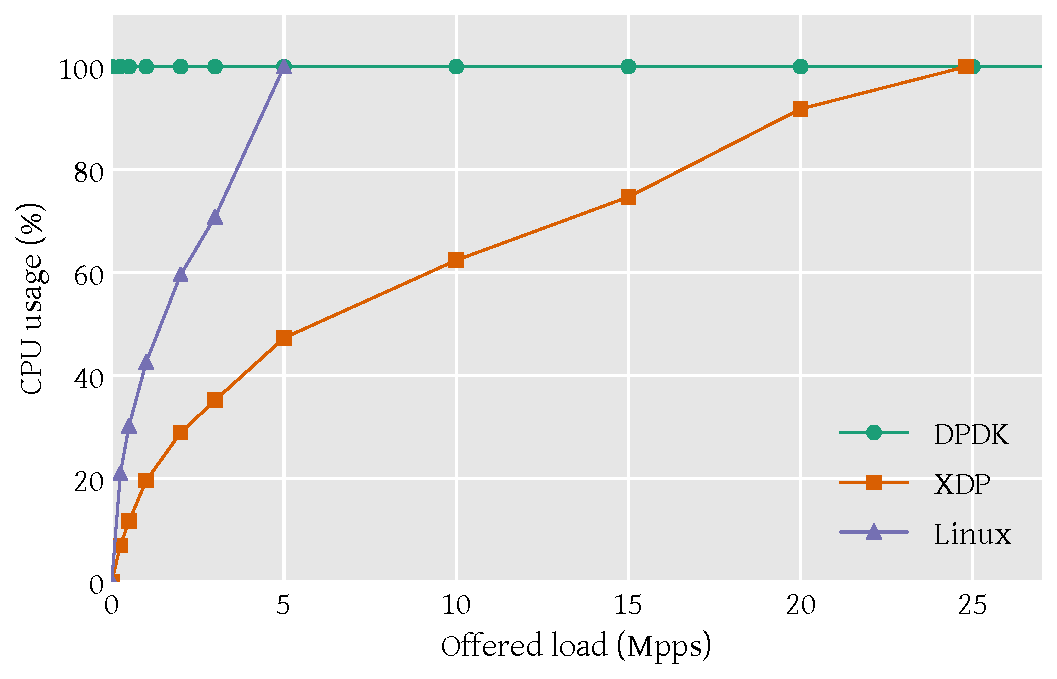
\includegraphics[width=\linewidth]{figures/drop-cpu.pdf}
\caption{\label{fig:drop-cpu} CPU usage in the drop scenario. Each line stops at
  the method's maximum processing capacity. The DPDK line continues at 100\% up
  to the maximum performance shown in Figure~\ref{fig:drop-test}.}
\end{figure}


\subsection{Packet Forwarding Performance}
\label{sec:pack-forw-perf}
Figure~\ref{fig:redirect-test} shows packet forwarding performance. The
forwarding applications perform a simple Ethernet address rewrite, where the
source and destination address of the incoming packet are swapped before the
packet is forwarded. This is the minimum rewriting that is needed for packet
forwarding to function, so the results represent an upper bound on forwarding
performance. Since XDP can forward packets out the same NIC as well as out a
different NIC (using two different program return codes), we include both modes
in the graph. The DPDK example program only supports forwarding packets through
a different interface, so we only include this operating mode in the test.
Finally, the Linux networking stack does not support this minimal forwarding
mode, but requires a full bridging or routing lookup to forward packets; this
lookup is expensive, and since the other applications do not perform it, the
results are not directly comparable. For this reason, we omit the Linux
networking stack from these results, and instead include the Linux routing
performance in our routing use case presented in Section~\ref{sec:fwd-usecase}.

As Figure~\ref{fig:redirect-test} shows, we again see linear scaling with the
number of cores up to a global performance bottleneck. The absolute performance
is somewhat lower than for the packet drop case, which shows the overhead of
packet forwarding. We also see that the XDP performance improves significantly
when packets are sent out on the same interface that they were received on,
surpassing the DPDK forwarding performance at two cores and above. The
performance difference is primarily due to differences in memory handling:
packet buffers are allocated by the device driver and associated with the
receiving interface. And so, when the packet is forwarded out a different
interface, the memory buffer needs to be returned to the interface that it is
associated with.

Looking at forwarding latency, as seen in Table~\ref{tbl:fwd-latency}, the
relative performance of XDP and DPDK for different-NIC forwarding are reflected
for the high packet rate test (with DPDK showing slightly lower variance as
well). However, for low packet rates, the latency of XDP is dominated by the
interrupt processing time, which leads to much higher end-to-end latency than
DPDK achieves with constant polling.

\begin{table}[tbp]
  \caption{\label{tbl:fwd-latency}Packet forwarding latency. Measurement machine
    connected to two ports on the same NIC, measuring end-to-end latency for 50
    seconds with high and low packet rates (100 pps and 1 Mpps).}
\centering
\begin{tabular}{lcccccc}
  \toprule
   & \multicolumn{2}{c}{Average}  &  \multicolumn{2}{c}{Maximum} &  \multicolumn{2}{c}{$< 10 \mu s$}  \\
   & \small 100 pps & \small 1 Mpps  &  \small 100 pps & \small 1 Mpps & \small 100 pps & \small 1 Mpps \\
  \midrule
  XDP & $82 \mu s$ & $7 \mu s$ & $272 \mu s$ & $202 \mu s$ & $0 \%$ & $98.1 \%$  \\
  DPDK & $2 \mu s$ &  $3 \mu s$ & $161 \mu s$ & $189 \mu s$ & $99.5 \%$ & $99.0 \%$  \\
\bottomrule
\end{tabular}
\end{table}

\begin{figure}[t]
\centering
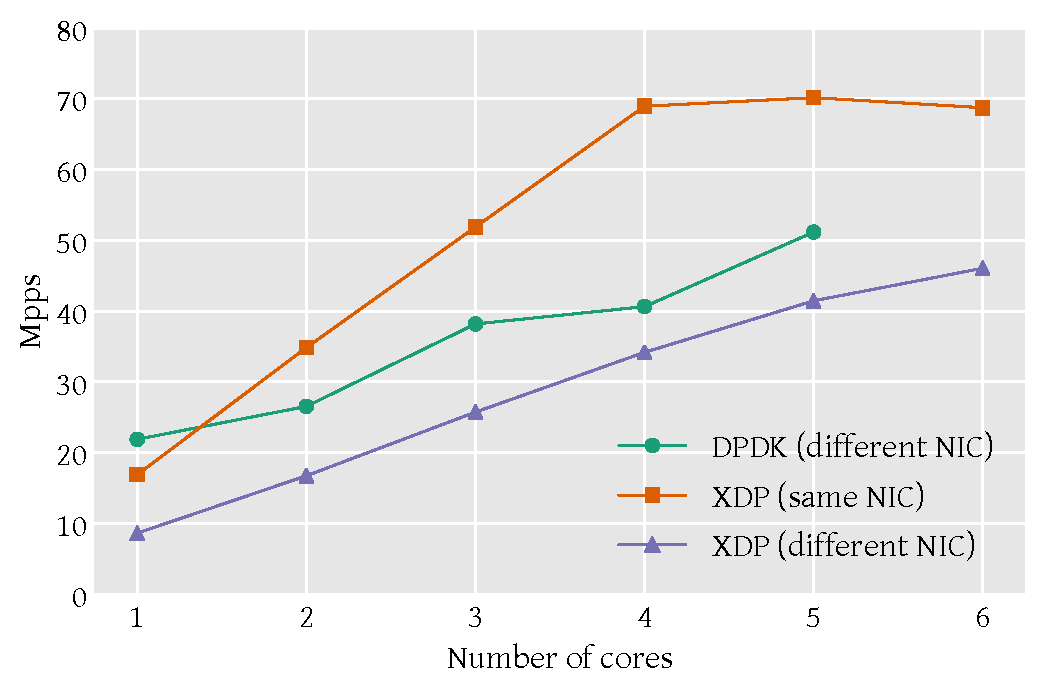
\includegraphics[width=\linewidth]{figures/redirect-test.pdf}
\caption{\label{fig:redirect-test} Packet forwarding throughput. Sending and
  receiving on the same interface takes up more bandwidth on the same PCI port,
  which means we hit the PCI bus limit at 70 Mpps.}
\end{figure}

\subsection{Discussion}
\label{sec:perf-discussion}

As we have seen in the previous subsections, XDP achieves significantly higher
performance than the regular Linux networking stack. Even so, for most use cases
XDP does not quite match the performance of DPDK. We believe this is primarily
because DPDK has incorporated more performance optimisations at the lowest level
of the code. To illustrate this, consider the packet drop example: XDP achieves
24\,Mpps on a single core, which corresponds to 41.6 nanoseconds per packet,
while DPDK achieves 43.5\,Mpps, or 22.9 nanoseconds per packet. The difference
of 18.7 nanoseconds corresponds to 67 clock cycles on the 3.6\,GHz processor in
our test machine. Thus, it is clear that every micro-optimisation counts; for
example, we measure an overhead of 1.3 nanoseconds for a single function call on
our test system. The mlx5 driver performs 10 function when processing a single
packet, corresponding to 13 of the 18.7 nanoseconds of performance difference
between XDP and DPDK.

Some of this overhead is inevitable on a general-purpose operating system such
as Linux, as device drivers and subsystems are structured in a way that makes it
possible to support a wide variety of systems and configurations. However, we
believe that some optimisations are viable. For instance, we have performed an
experiment that removed DMA-related function calls that were not needed on our
specific hardware from the driver (removing four of the 10 per-packet function
calls), which improved the packet drop performance to 29\,Mpps. We see similar
effects with other drivers, such as the \emph{i40e} driver for 40\,Gbps Intel
cards, which has a smaller performance delta between XDP and
DPDK.\footnote{While DPDK uses the drivers in the operating system to assume
  control of the hardware, it contains its own drivers that are used for the
  actual packet processing.}

Given the above points, we believe it is feasible for XDP to further decrease
the performance delta to DPDK. However, given the benefits of XDP in terms of
flexibility and integration with the rest of the system, XDP is already a
compelling choice for many use cases; we show some examples of this in the next
section.

\section{Real-world use cases}
\label{sec:usecases}
To show how the various aspects of XDP can be used to implement useful
real-world applications, this section describes three example use cases. These
use cases have all seen deployment in one form or another, although we use
simplified versions in our evaluation to be able to make the code available. We
also refer the reader to~\cite{miano2018creating} for an independent look at
some of the challenges of implementing real-world network services in XDP.

Our first use case shows how XDP's kernel helper functions can be used to
accelerate common use cases, using the example of a software router. In the
second use case, we show how an inline Denial of Service (DoS) mitigation
application can be used to protect against attacks directly at the application
server. And finally, the third use case shows how the forwarding mode that sends
packets out the same interface as they arrived on can be used to implement a
layer-4 load balancer.

As mentioned in Section~\ref{sec:perf-eval}, the purpose of this section is to
demonstrate the feasibility of implementing the selected use cases in XDP, not
to perform an exhaustive performance evaluation against state of the art
implementations of each use case. Instead, we use the regular Linux kernel stack
as a simple performance baseline and benchmark the XDP applications against
that.

\subsection{Software Routing}
\label{sec:fwd-usecase}
The Linux kernel contains a full-featured routing table, which includes support
for policy routing, source-specific routing, multi-path load balancing, and more.
For the control plane, routing daemons such as Bird~\cite{bird} or
FRR~\cite{frr} implement a variety of routing control plane protocols. Because
of this rich ecosystem supporting routing on Linux, re-implementing the routing
stack in another packet processing framework carries a high cost, and improving
performance of the kernel data plane is desirable.

XDP is a natural fit for this task, especially as it includes a helper function
which performs full routing table lookups directly from XDP. The result of the
lookup is an egress interface and a next-hop MAC address, which makes it
possible for the XDP program to immediately forward the packet if the lookup
succeeds. If no next-hop MAC is known (because neighbour lookup has not been
performed yet), the XDP program can pass the packet to the networking stack,
which will resolve the neighbour, allowing subsequent packets to be forwarded by
XDP.

To show the performance of this use case, we use the XDP routing example that is
included in the Linux kernel source~\cite{fwd-example} and compare its
performance to routing in the regular Linux network stack. We perform two tests:
one with a single route installed in the routing table, and another where we use
a full dump of the global BGP routing table from \emph{\url{routeviews.org}}. In
both cases, all next-hop addresses are set to the address of the test system
connected to our egress interface. The full table contains 752,138 distinct
routes, and for our tests we generate 4000 random destination IP addresses to
make sure we exercise the full table.\footnote{Using fewer than 4000 destination
  IPs, the part of the routing table that is actually used is small enough to be
  kept in the CPU cache, which gives misleading (better) results. Increasing the
  number of IPs above 4000 had no additional effects on forwarding
  performance.}.

The performance of this use case is seen in Figure~\ref{fig:router-fwd}. Using
XDP for the forwarding plane improves performance with a factor of 2.5 for a
full table lookup, and a factor of 3 for the smaller routing table example. This
makes it feasible to run a software router with a full BGP table at line rate on
a 10\,Gbps link using a single core (using a conservative estimate of an average
packet size of 300\,bytes).

\begin{figure}[t]
\centering
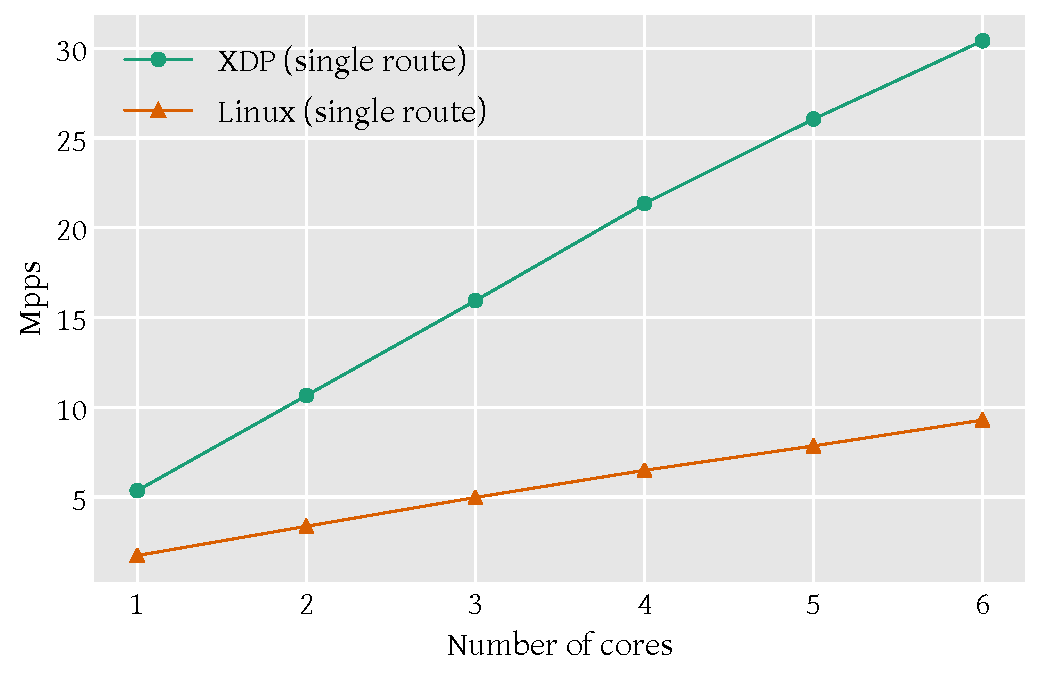
\includegraphics[width=\linewidth]{figures/router-fwd.pdf}
\caption{\label{fig:router-fwd} Software routing performance. Since the
  performance scales linearly with the number of cores, only the results for a
  single core are shown.}
\end{figure}

% See: (calc in benchmarks/bench04_fwd.org). The full-tables vs. single overhead
%  is significantly larger than the expected overhead (according to Vincent
%  Bernat's measurements)
%  https://vincent.bernat.im/en/blog/2017-performance-progression-ipv4-route-lookup-linux

\subsection{Inline DoS Mitigation}
\label{sec:dos-usecase}
DoS attacks continue to plague the internet, typically in the form of
distributed attacks (DDoS attacks) from compromised devices. With XDP, it is
possible to deploy packet filtering to mitigate such attacks directly at the
application servers, without needing to change applications. In the case of a
virtual machine deployment, the filter can even be installed in the hypervisor,
and thus protect all virtual machines running on the host.

To show how this could work, we perform a test modelled on the DDoS mitigation
architecture used by Cloudflare, which uses XDP as the filtering
mechanism~\cite{cloudflare-ddos}. Their Gatebot architecture works by sampling
traffic at servers located in distributed Points of Presence (PoPs), collecting
it centrally for analysis, and formulating mitigation rules based on the
analysis. The mitigation rules take the form of a series of simple checks on the
packet payload, which are compiled directly into eBPF code and distributed to
the edge servers in the PoPs. Here the code is executed as an XDP program that
will drop packets matching the rules, while also updating match counters stored
in BPF maps.

To test the performance of such a solution, we use an XDP program that parses
the packet headers and performs a small number of tests\footnote{Our example
  program performs four packet data reads per packet, to parse the outer packet
  headers and drop packets with a pre-defined UDP destination port number.} to
identify attack traffic and drop it, and uses the CPU redirect feature to pass
all other packets to a different CPU core for processing. To simulate a baseline
application load we use the Netperf benchmarking tool~\cite{netperf}. Netperf
contains a TCP-based round-trip benchmark, which opens a TCP connection and
sends a small payload that is echoed back from the server, repeating as soon as
a reply is received. The output is the number of transactions per second, which
represents performance of an interactive use case, such as small remote
procedure calls.

We run our experiment on a single core, to illustrate the situation where
legitimate traffic has to compete for the same hardware resources as attack
traffic. We apply a baseline load of 35.000 TCP transactions per second, then
simulate the DoS attack by offering an increasing load of small UDP packets
matching our packet filter. We measure the TCP transactions performance as the
attack traffic volume increases, reporting the average of four test repetitions
per data point.

\begin{figure}[t]
\centering
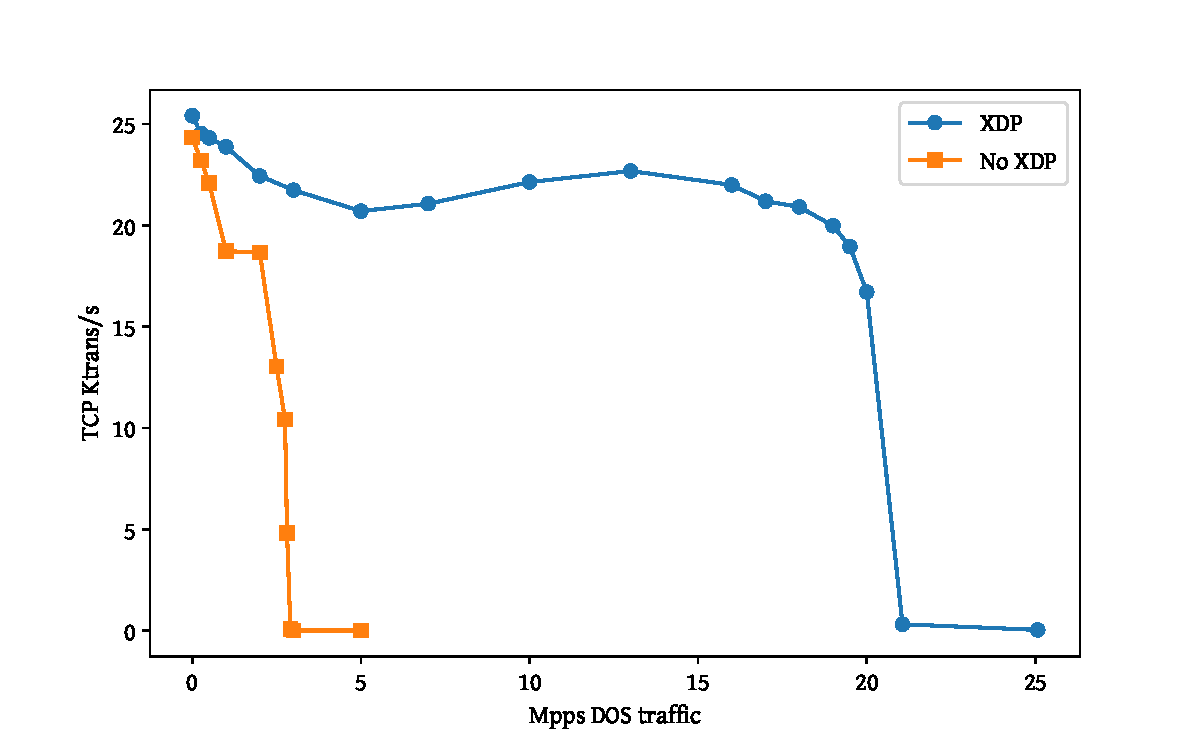
\includegraphics[width=\linewidth]{figures/ddos-test.pdf}
\caption{\label{fig:ddos-results} DDoS performance. Number of TCP transactions
  per second as the level of attack traffic directed at the server increases.}
\end{figure}

The results of this is shown in Figure~\ref{fig:ddos-results}. Without the XDP
filter, performance drops rapidly, being halved at 3\,Mpps and effectively zero
at just below 3.5\,Mpps of attack traffic. However, with the XDP filter in
place, the TCP transaction performance is stable at around 28.500 transactions
per second until 19.5\,Mpps of attack traffic, after which it again drops
rapidly. This shows that effective DDoS filtering is feasible to perform in XDP,
which comfortably handles 10\,Gbps of minimum-packet DoS traffic on a single CPU
core. Deploying DDoS mitigation this way leads to increased flexibility, since
no special hardware or application changes are needed.

\subsection{Load Balancing}
\label{sec:load-balancer}
For the load balancer use case, we use the XDP component of the Katran load
balancer~\cite{katran} recently released as open source by Facebook. This works
by announcing an IP address for the service, which is routed to the load
balancer. The load balancer hashes the source packet header to select a
destination application server. The packet is then encapsulated and sent to the
application server, which is responsible for decapsulating it, processing the
request, and replying directly to the originator. The XDP program performs the
hashing and encapsulation, and returns the packet out the same interface on
which it was received. It keeps state in BPF maps and implements the
encapsulation entirely in the eBPF program.

To test this use case, we configure the Katran XDP program with a fixed number
of destination hosts\footnote{We use one virtual IP per CPU core, and 100
  destinations per virtual IP.}, and run it on our test machine. We compare it
with the IPVS load balancer that is part of the Linux kernel, which can be
configured in the same way. The performance of both is shown in
Table~\ref{tbl:load-balancer}, which shows linear scaling with the number of
CPUs, and that XDP offers a performance gain of 4.3x over IPVS.

\begin{table}[tbp]
\caption{\label{tbl:load-balancer}Load balancer performance (Mpps).}
\centering
\begin{tabular}{lcccccc}
  \toprule
  CPU Cores & 1   &  2  &  3  &  4  &  5  &  6  \\
  \midrule
  XDP (Katran) & 5.2 & 10.1 & 14.6 & 19.5 & 23.4 & 29.3 \\
  Linux (IPVS) & 1.2 & 2.4 & 3.7 & 4.8 & 6.0 & 7.3 \\
\bottomrule
\end{tabular}
\end{table}


\section{Limitations and future work}
\label{sec:limitations}
As we have shown above, XDP offers high performance and can be used to implement
a variety of real-world use cases. However, this does not mean that XDP is a
finished system. On the contrary, as part of the Linux kernel, XDP undergoes
continuous improvement. Some of this development effort goes into softening the
rough edges that are the inevitable result of XDP being incrementally
incorporated into a general purpose operating system kernel. Other efforts
continue to push the boundaries of XDP's capabilities. In this section we give
an overview of some of these efforts.

\subsection{Limitations on eBPF programs}
\label{sec:limit-ebpf-progr}

As mentioned previously, the programs loaded into the eBPF virtual machine are
analysed by the eBPF verifier, which places certain limitations on the programs
to ensure they do not harm the running kernel. These limitations fall in two
categories: (a) Ensuring the program will terminate, which is implemented by
disallowing loops and limiting the maximum size of the program. And (b) ensuring
the safety of memory accesses, which is done by the register state tracking
explained in Section~\ref{sec:bpf-verifier}.

The primary function of the verifier is to ensure the safety of the kernel from
programs being loaded into it. As such, a conservative approach is taken, where
the verifier will reject any program that it cannot prove is safe. This can lead
to false negatives, where safe programs are needlessly rejected. In addition, as
others have noted~\cite{miano2018creating}, the restrictions on the program
structure imposed by the verifier, such as the lack of support loops, have been
more limited than strictly necessary, in the interest of ensuring safety. To
improve upon this situation, there is an ongoing effort to reduce false
negatives, i.e., cases where the verifier rejects programs that are actually
safe to run. Furthermore, the error messages reported by the verifier have been
made friendlier, to make it easier for developers to change their code to avoid
verification errors. Support for function calls in eBPF has recently been added,
the addition of support for bounded loops is planned, and efficiency
improvements that will allow the verifier to operate on larger programs are
being worked on.

Another limitation of eBPF programs compared to user-space C programs is the
lack of a standard library, including things like memory allocation, threading,
locking, etc. This is partly alleviated by the life cycle and execution context
management of the kernel (i.e., an XDP program is automatically run for each
arriving packet), and partly by the helper functions exposed by the kernel.

Finally, only one XDP program can be attached to each networking interface. This
can be worked around by cooperation between programs, where the tail call
functionality can be used to either dynamically dispatch to different programs
depending on packet content, or to chain several programs together to operate in
sequence.

\subsection{User Experience and Debugging}
\label{sec:user-exper-debugg}
Since an XDP program runs in the kernel, the debugging tools available to a
regular userspace program are not generally applicable. Instead, the debugging
and introspection features included in the kernel can be applied to XDP (and
other eBPF programs). These tools include tracepoints and
kprobes~\cite{kernel-tracing} as well as the performance counters that are part
of the \emph{perf} subsystem~\cite{perf}. However, developers who are not
familiar with the kernel ecosystem may find this ecosystem of kernel-specific
tools a limitation. To ease the transition, a variety of tools exist, including
the BPF Compiler Collection~\cite{bcc}, the \emph{bpftool} introspection
program~\cite{bpftool} and the \emph{libbpf} library of utility
functions~\cite{libbpf}. These have already seen significant improvements, but
more work is needed in this area.


\subsection{Driver Support}
\label{sec:driver-support}
Each device driver needs to add support for running XDP programs, by supporting
an API exposed by the core networking stack. Support is continuously being added
to more and more drivers,\footnote{At the time of writing Linux 4.18 has XDP
  support in 12 different drivers, including most high-speed network adapters.
  For an updated list, see~\cite{cilium-docs}.} but some care is still needed
when selecting hardware to use with XDP. However, since XDP is integrated into
the kernel device driver model, it imposes no particular capability constraints
on the hardware, which means that full support in all drivers is possible.

As the XDP system has evolved, the need to keep the changes required in drivers
to support XDP to a minimum has become increasingly clear, and some steps have
been taken in this direction. For instance, support for new targets can be added
to the redirection action without any changes needed from the drivers. Finally,
the Generic XDP feature~\cite{generic-xdp} allows running XDP programs (at
reduced performance) even if the networking driver lacks the proper support, by
moving execution into the core networking stack.

\subsection{Performance Improvements}
\label{sec:perf-improvements}
As we discussed in Section~\ref{sec:perf-discussion}, there is still a
performance gap between XDP and DPDK in some use cases. Efforts to improve this
are ongoing, which includes micro-optimisations of driver code as well as
changes to the core XDP code to avoid unnecessary operations where possible, and
otherwise amortise the costs through improved batching of operations.

\subsection{QoS and Rate Transitions}
\label{sec:handl-rate-trans}
Currently, XDP does not implement any mechanism for supporting different Quality
of Service (QoS) levels. Specifically, an XDP program receives no back-pressure
when attempting to forward packets to a destination that has exhausted its
capacity, such as when joining networks with different speeds or other
mismatched network characteristics.

While QoS is lacking from XDP, the Linux kernel networking stack features
best-in-class Active Queue Management (AQM) and packet scheduling
algorithms~\cite{good-bad-wifi}. Not all of these features are a good fit for
the XDP architecture, but we believe that selectively integrating features from
the networking stack into XDP is an opportunity to provide excellent support for
QoS and AQM in XDP, in a way that can be completely transparent to the packet
processing applications themselves. We are planning to explore this further.

\subsection{Accelerating Transport Protocols}
\label{sec:accel-transp-prot}

With XDP we have shown how high-speed packet processing can be integrated
cooperatively into the operating system to accelerate processing while making
use of existing features of the operating system where it makes sense. XDP
focuses on stateless packet processing, but extending the same model to stateful
transport protocols such as TCP would provide many of the same performance
benefits to applications that require reliable (and thus stateful) transports.
Indeed, others have shown that accelerated transport protocols can significantly
improve performance relative to the regular operating system
stack~\cite{stackmap,sandstorm,belay2014ix,jeong2014mtcp}.

One of these previous solutions~\cite{stackmap} shows that there is significant
potential in improving the raw packet processing performance while keeping the
in-kernel TCP stack itself. XDP is a natural fit for this, and there has been
some initial discussion of how this could be achieved~\cite{txdp}; while far
from trivial, this presents an exciting opportunity for expanding the scope of
the XDP system.

\subsection{Zero-copy to userspace}
\label{sec:zero-copy-userspace}

As mentioned in Section~\ref{sec:prog-model}, an XDP program can redirect data
packets to a special socket opened by a user space application. This can be used
to improve performance of network-heavy applications running on the local
machine. However, in its initial implementation, this mechanism still involves
copying the packet data, which negatively affects performance. There is ongoing
work to enable true zero-copy data transfer to user space applications through
\texttt{AF\_XDP} sockets. This places some constrains on the memory handling of
the network device, and so requires explicit driver support. The first such
support was merged into the kernel in the 4.19 release cycle, and work is
ongoing to add it to more drivers. The initial performance numbers look
promising, showing transfers of upwards of 20 Mpps to userspace on a single
core.

\subsection{XDP as a building block}
\label{sec:xdp-building-block}

Just as DPDK is used as a low-level building block for higher level packet
processing frameworks (e.g., \cite{linguaglossa2017high}), XDP has the potential
to serve as a runtime environment for higher-level applications. In fact, we
have already started to see examples of applications and frameworks leveraging
XDP. Prominent examples include the Cilium security middle-ware~\cite{cilium},
the Suricata network monitor~\cite{suricata} and the P4-to-XDP compiler
project~\cite{p4xdp}.

\section{Conclusions}
\label{sec:conclusion}
We have presented XDP, a system for safely integrating fast programmable packet
processing directly into the operating system kernel. Our evaluation has shown
that XDP achieves raw packet processing performance of up to 24 million packets
per second on a single CPU core.

While this is not quite on par with state of the art kernel bypass-based
solutions, we argue that XDP offers other compelling features that more than
make up for the performance delta. These features include retaining kernel
security and management compatibility; selectively utilising existing kernel
stack features as needed; providing a stable programming interface; and complete
transparency to applications. In addition, XDP can be dynamically re-programmed
without service interruption, and requires neither specialised hardware nor
dedicating whole CPU cores to packet processing.

We believe that these features make XDP a compelling alternative to
all-or-nothing kernel bypass solutions. This belief is supported by XDP's
adoption in a variety of real-world applications, some of which we have shown
examples of above. Furthermore, the XDP system is still evolving, and we have
outlined a number of interesting developments which will continue to improve it
in the future.

\section*{Acknowledgements}
\label{sec:acknowledgements}
XDP has been under development by the Linux networking community for a number of
years, and the authors would like to thank everyone who has been involved in
this process. In particular, Alexei Starovoitov has been instrumental in the
development of the eBPF virtual machine and verifier, Jakub Kicinski has been a
driving force behind XDP hardware offloading and development of the bpftool
utility, and Björn Töpel plus Magnus Karlsson have been leading the AF\_XDP and
userspace zero-copy efforts.


\bibliographystyle{ACM-Reference-Format}
\bibliography{xdp}

\end{document}

% Local Variables:
% TeX-command-extra-options: "-shell-escape"
% End:
